\chapter{\IfLanguageName{dutch}{Stand van zaken}{State of the art}}
\label{ch:stand-van-zaken}

% Tip: Begin elk hoofdstuk met een paragraaf inleiding die beschrijft hoe
% dit hoofdstuk past binnen het geheel van de bachelorproef. Geef in het
% bijzonder aan wat de link is met het vorige en volgende hoofdstuk.

% Pas na deze inleidende paragraaf komt de eerste sectiehoofding.

In de inleiding is duidelijk geworden dat het onderzoek gericht zal zijn op twee mogelijke dataformaten aan de hand van 2 verschillende structuren, namelijk JSON aan de hand van REST en gRPC aan de hand van Protocol Buffers. Om dit onderzoek volledig te kunnen begrijpen is het belangrijk om de werking en de basisprincipes van deze dataformaten en de daarbij behorende structuren te begrijpen. Om deze reden zal eerst kort uitgelegd worden wat een API is, vervolgens zal de werking en basisprincipes van JSON en RESTful API uitgelegd worden, en als volgt die van gRPC en Protocol Buffers. Alsook wordt de interne werking van de architectuur van de Fashion Society uitgelegd aan de hand van de gebruikte ontwerppatronen en een praktisch voorbeeld.

\section{API}
\label{sec:API}

\subsection{Wat is een API?}
\label{subsec:Wat is een API?}

Een API of Application Programming Interface is een programma dat wordt gebruikt als tussenlaag die het mogelijk maakt voor twee applicaties om met elkaar te communiceren \autocite{HubSpire}. Meer in detail is het een interface die de interacties tussen meerderere applicaties, bestaande uit zowel hardware als software, gaat vastleggen. Deze interacties zijn in de vorm van requests, de interface legt vast hoe deze requests moeten afgehandeld worden, welke dataformaten gebruikt moeten worden, welke richtlijnen en conventies er gevolgd moeten worden etc.

Daarnaast kan een API op verschillende manieren ontworpen worden, volledig op maat, specifiek voor een bepaalde applicatie of component of op basis van een standaard om interoperabiliteit te kunnen garanderen.

\subsection{Hoe werkt een API?}
\label{subsec:Hoe werkt een API?}

Een API communiceert op basis van vooropgestelde regels die bepalen hoe applicaties en machines met elkaar kunnen communiceren. In dit proces is de API een tussenlaag tussen twee applicaties of machines dat met elkaar willen connecteren voor een specifieke taak.

Een simpel voorbeeld hiervan is het opzoeken van gegevens in Google Search. In de webpagina wordt een zoekterm opgegeven en eens er op de zoekknop gedrukt wordt of op enter gedrukt wordt dan stuurt de webpagina een request naar de achterliggende API die vervolgens op de servers alle gerelateerde data gaat ophalen en terug weergeven aan de webpagina.

\subsection{Verschillende API types}
\label{subsec:Verschillende API types}

Voor het onderzoek wordt er gebruik gemaakt van Web APIs, dit zijn APIs die gecontacteerd kunnen worden aan de hand van het HTTP protocol. Dit soort APIs kunnen we onderverdelen in vier categoriëen \autocite{Stoplight}.

\textbf{Open APIs}

Open APIs staan ook wel bekend als publieke APIs, dit zijn APIs die toegankelijk zijn met minimale restricties voor vrijwel iedereen. Mogelijks kan een Open API registratie vereisen of het gebruik van een API key. Dit soort APIs hebben als doel om data of services toegankelijk te maken voor externe gebruikers.

\textbf{Interne APIs}

Interne APIs zijn APIs die gebruikt worden binnen een bepaald bedrijf voor intern resources te kunnen delen zoals data en services. Op deze manier kunnen verschillende diensten of teams binnen éénzelfde bedrijf elkaars resources gebruiken. Voordelen van interne APIs zijn beveiliging en een gestandariseerde interface voor het connecteren van meerdere services.

\textbf{Partner APIs}

Partner APIs zijn gelijkend aan Open APIs, echter zitten hier veel meer restricties op en worden deze gecontrolleerd door een API Gateway (hoofdstuk \ref{subsec:API-gateway patroon}). Deze APIs worden het meest gebruikt voor doeleinden zoals het toegang verlenen tot betalende services en worden vaak gebruikt in Software as a Service.

\textbf{Samengestelde APIs}

De samengestelde APIs laten het toe om meerdere endpoints te contacteren aan de hand van één request. Dit soort APIs zijn vooral handig in microservice architecturen (hoofdstuk \ref{subsec:Microservice architectuur patroon}) in situaties waar data nodig is van meerdere services om één specifieke taak uit te voeren. Het gebruik van dit soort APIs kan voordelen opleveren zoals een vermindering in server load en verbetering van de performantie van een applicatie.

\section{JSON}
\label{sec:JSON}

\subsection{Algemeen}
\label{subsec:Algemeen}

JSON is een dataformaat zoals bijvoorbeeld XML en de afkorting staat voor JavaScript Object Notation. JSON is beschreven in Standard ECMA-404 ~\autocite{Json2017} en is een structuur van accolades, haakjes, dubbele punten en komma's die zeer nuttig kunnen zijn in verschillende contexten, profielen en applicaties. Een voorbeeld hiervan is te zien in figuur \ref{fig:jsonExample}.

\begin{figure}[H]
    \centering
    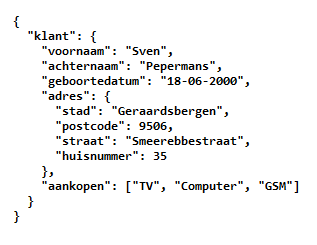
\includegraphics[scale=1.50]{jsonExample}
    \caption[JSON Example]{Een voorbeeld van een JSON.}
    \label{fig:jsonExample}
\end{figure}

JSON mag niet gezien worden als een specificatie van een gegevensuitwisseling. Bij een zinvolle gegevensuitwisseling wordt er een overeenstemming over de structuur die gekoppeld is aan een gebruik van JSON tussen producent en consument vereist. JSON kan wel gezien worden als een syntactisch raamwerk waaraan een specifieke structuur kan worden gekoppeld.

Doordat er veel verschillende types getallen zijn zoals decimale en binaire getallen, kiest JSON enkel voor een weergave van getallen die mensen gebruiken, namelijk een reeks cijfers. Ook al zijn alle programmeertalen het niet altijd eens over de interne representaties van getallen, ze weten wel hoe ze cijferreeksen moeten begrijpen.

 Objecten kunnen op veel verschillende manieren voorgesteld worden, met andere woorden kunnen de modellen van objecten heel erg uiteenlopen. Om dit probleem aan te pakken biedt JSON een eenvoudige notatie aan voor het uitdrukken van verzamelingen met naam / waarde-paren. Om zulke verzamelingen weer te geven hebben de meeste programmeertalen reeds een functie zoals struct, map, hash en object.
Daarnaast biedt JSON ook ondersteuning voor geordende zoeklijsten, alsook hiervoor hebben alle programmeertalen een functie om deze weer te geven zoals array, vector en list. Aangezien objecten en arrays zich kunnen nesten, kunnen aan de hand van JSON complexe structuren zoals boomstructuren worden gerepresenteerd.

Hieruit kan worden geconcludeerd dat door het aanvaarden van JSON's simpele conventies, complexe datastructuren uitgewisseld kunnen worden tussen wat anders incompatiebele programmeertalen zijn.



\subsection{JSON in detail bekeken}
\label{subsec:JSON in detail bekeken}

Een JSON-tekst bestaat uit een reeks tokens die gevormd zijn uit Unicode-codepunten en die in overeenstemming zijn met de achterliggende JSON grammatica. Zo een reeks tokens bevat tekenreeksen, cijfers, zes structurele tokens en drie letterlijke naamtokens.
Hieronder volgt een opsomming van de zes structurele tokens en de drie literal name tokens.

De zes structurele tokens:

\begin{itemize}
    \item $\rbrack$ Linker vierkante haak
    \item $\rbrack$ Rechter vierkante haak
    \item \{ Linker accolade
    \item \} Rechter accolade
    \item : Dubbele punt
    \item , Komma
\end{itemize}

De drie literal name tokens:

\begin{itemize}
    \item true  
    \item false     
    \item null      
\end{itemize}

Voor of na de meeste tokens is het toegestaan om witruimte te gebruiken, maar niet binnen in een token zelf, een spatie is hierop een uitzondering en is wel toegestaan in strings. deze witruimte kan beschreven worden als een willekeurige reeks van één of meerdere van onderstaande codepunten.

\begin{itemize}
    \item Character tabulation       
    \item Line feed       
    \item Carriage return   
    \item Spatie           
\end{itemize}


\subsection{Waarden}
\label{subsec:Waarden}

De bovengestelde tokens vormen de ruggengraat van een JSON-bestand, echter is het de bedoeling dat een JSON-bestand data overdraagt. Deze data kan aan de hand van verschillende waarden worden voorgesteld, namelijk als objecten, arrays, nummers, strings, true, false en null. Alle mogelijke waarden zijn zichtbaar in figuur \ref{fig:jsonValue}.

\begin{figure}[ht]
    \centering
    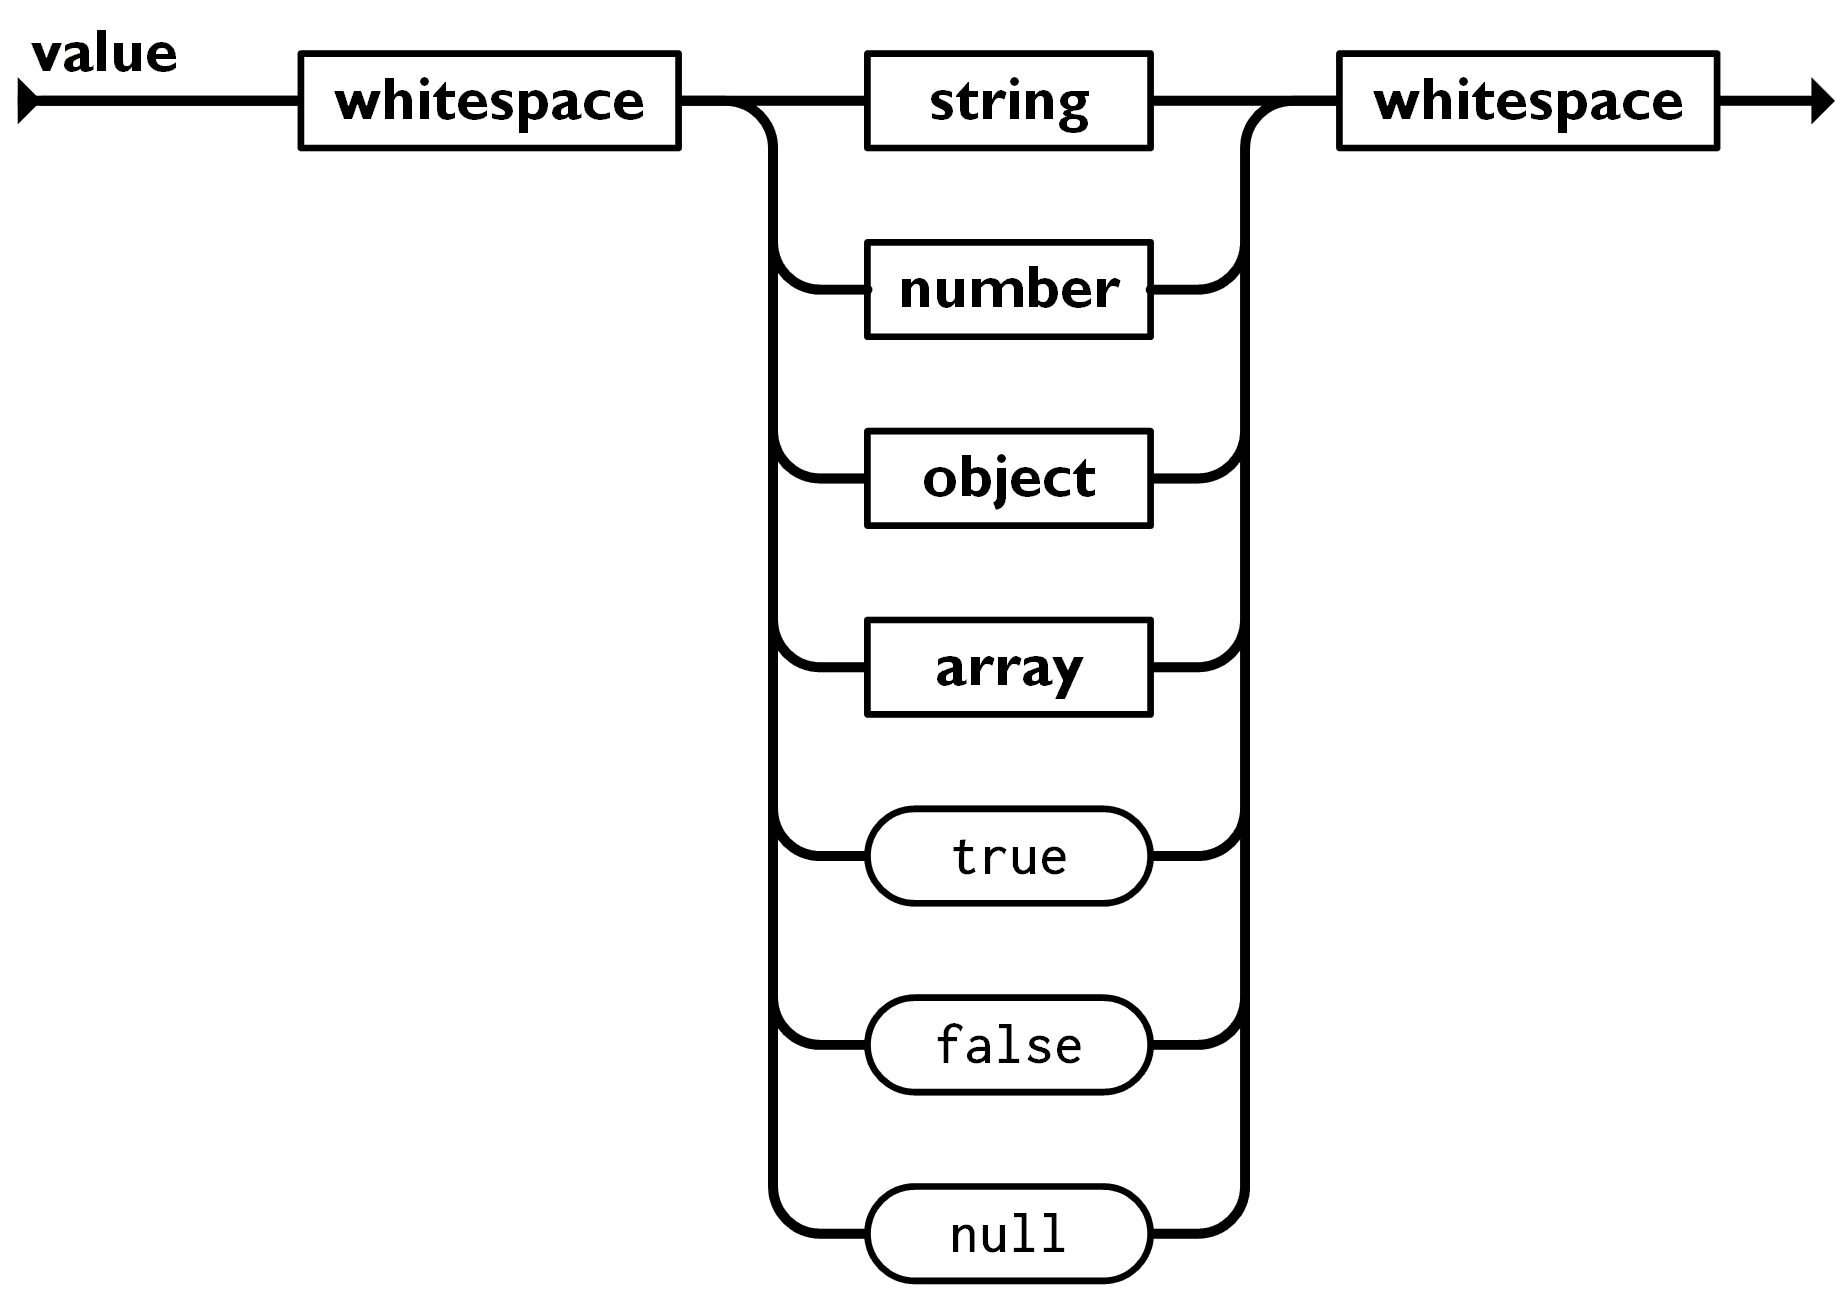
\includegraphics[scale=0.75]{jsonValue}
   \caption[JSON values]{De structuur van een JSON-waarde met alle mogelijke waarden die deze kan bevatten. \autocite{Crockford}}
   \label{fig:jsonValue}
\end{figure}

De eerste waarden die besproken worden zijn de objecten, deze worden voorgesteld door een paar accolades die geen of meerdere name/value paren kunnen omringen zoals te zien is in figuur \ref{fig:jsonObject} en in figuur \ref{fig:objectEx}. In een name/value paar is de naam een string en wordt gevolgd door een dubbele punt die de naam en waarde van elkaar onderscheidt. 
Na de waarde kan optioneel een komma gezet worden, deze onderscheidt de waarde en de volgende naam van elkaar. Tot slot moeten de namen niet uniek zijn en moeten ze geen bepaalde ordening volgen.

\begin{figure}[H]
    \centering
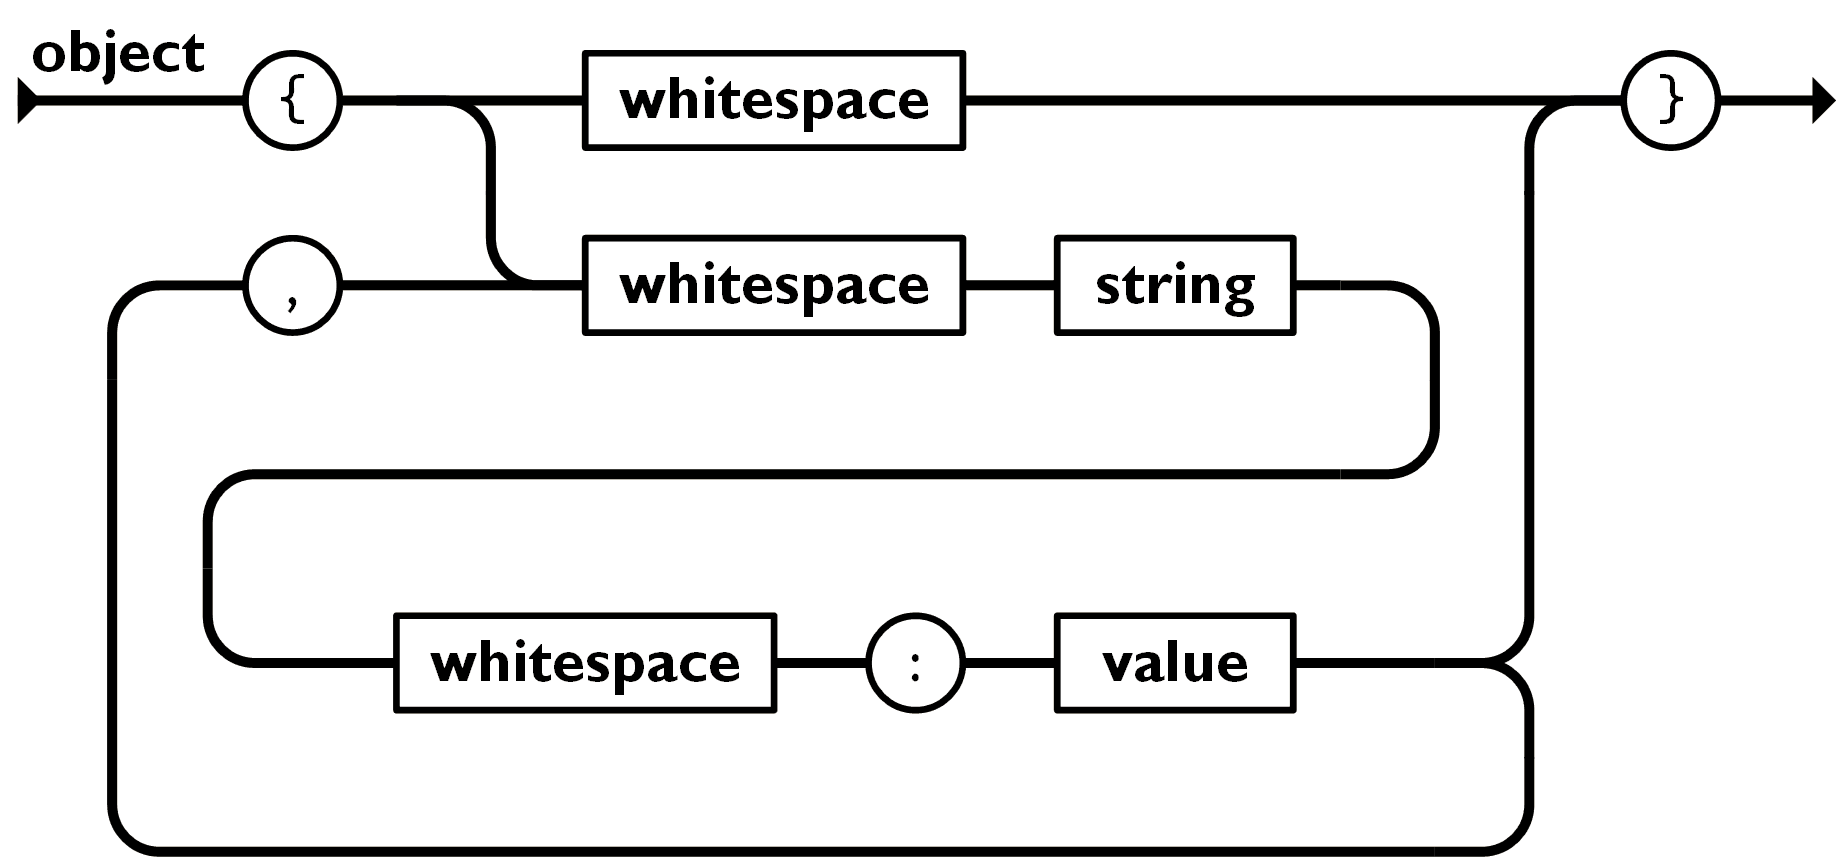
\includegraphics[scale=0.75]{jsonObject}
\caption[JSON Object Structuur]{De structuur van een JSON object. \autocite{Crockford}}
    \label{fig:jsonObject}
\end{figure}

\begin{figure}[H]
    \centering
    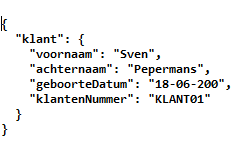
\includegraphics[scale=1.5]{objectEx}
    \caption[JSON Object]{Voorbeeld van een JSON object.}
    \label{fig:objectEx}
\end{figure}

Een tweede waarde zijn de arrays, dit zijn vierkante haken die geen of meerdere waarden omringen. Het bijzondere aan arrays is dat deze niet beperkt zijn tot een name/value paar en dus ook andere arrays kunnen bevatten en genest kunnen worden. Dit kan afgeleid worden uit figuur \ref{fig:jsonArray}. De array structuur wordt net zoals bij objecten geen beperkingen opgelegd, echter worden deze vooral gebruikt in situaties waar de ordening wel enig belang heeft. Figuur \ref{fig:arrayEx} is hier een duidelijk voorbeeld van.

\begin{figure}[H]
    \centering
    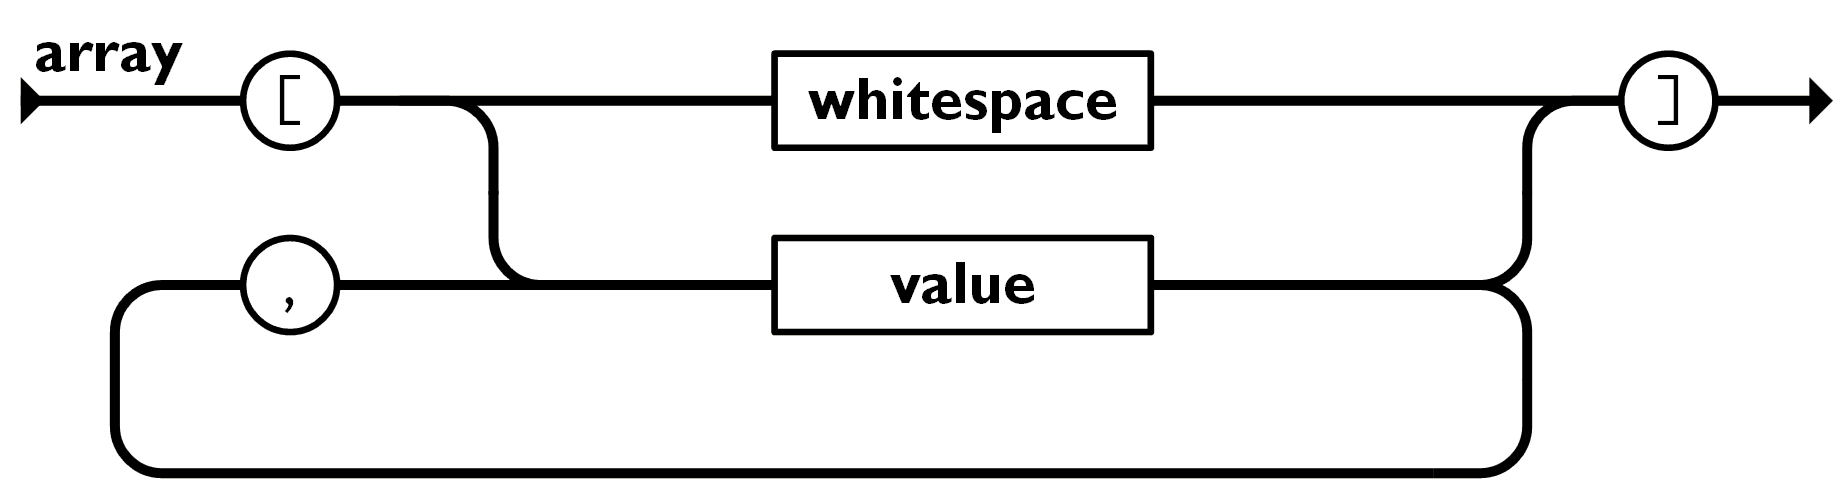
\includegraphics[scale=0.75]{jsonArray}
    \caption[JSON Array Structuur]{De structuur van een JSON array.\autocite{Crockford}}
    \label{fig:jsonArray}
\end{figure}
\begin{figure}[H]
    \centering
    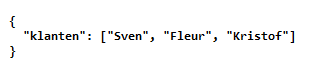
\includegraphics[scale=1.50]{arrayEx}
    \caption[JSON Array]{Een voorbeeld van een JSON Array.}
    \label{fig:arrayEx}
\end{figure}

Vervolgens zijn er de nummers, een nummer kan gedefinieerd worden als een sequentie van decimale cijfers. Bij deze sequentie cijfers is er geen overbodige voorloopnul, een nummer kan wel voorafgegaan worden door een min-teken, als ook kan een nummer voorafgegaan worden door zowel een kleine als een grote e om een exponent aan te duiden dat  eventueel kan worden bijgestaan door een plus- of min-teken. Om te werken met kommagetallen wordt een decimaal punt gebruikt. Deze structuur is te zien in figuur \ref{fig:jsonNumber} en een voorbeeld hiervan in figuur \ref{fig:numberEx}.

\begin{figure}[H]
    \centering
    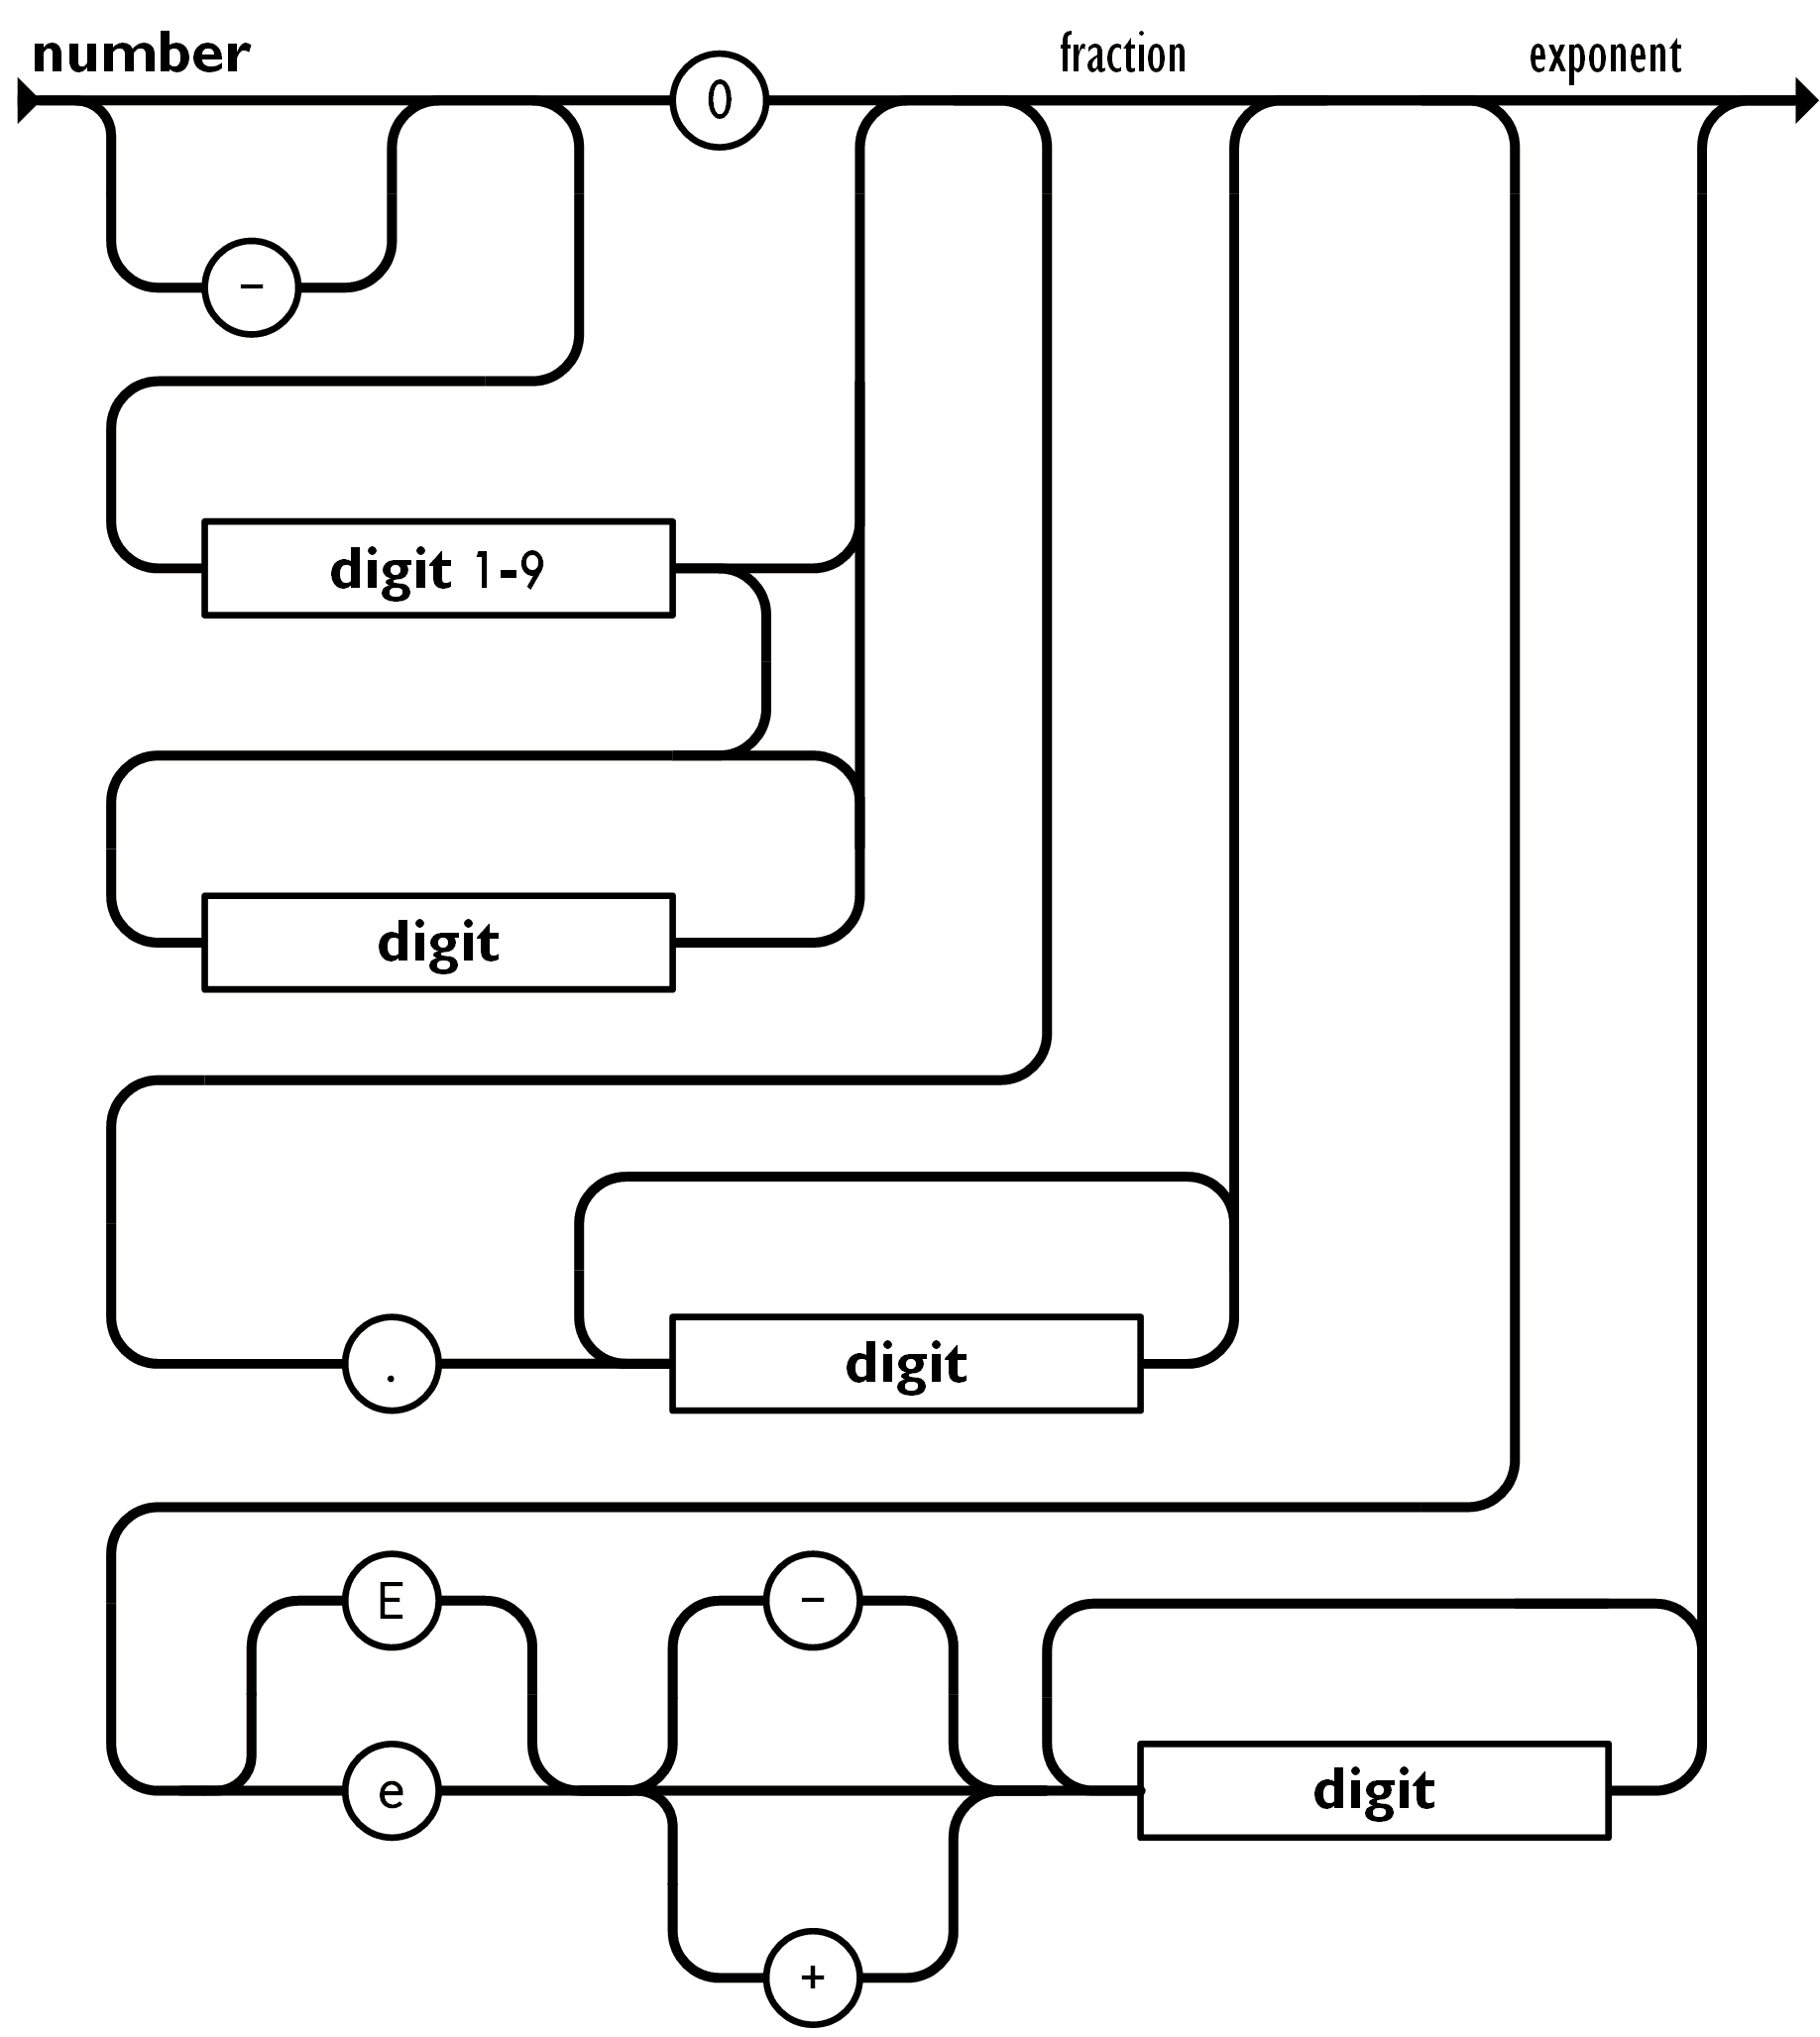
\includegraphics[scale=0.7]{jsonNumber}
    \caption[JSON Nummer Structuur]{De structuur van een JSON nummer. \autocite{Crockford}}
    \label{fig:jsonNumber}
\end{figure}

\begin{figure}[H]
    \centering
    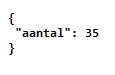
\includegraphics[scale=1.50]{numberEx}
    \caption[JSON Nummer]{Een voorbeeld van een JSON nummer.}
    \label{fig:numberEx}
\end{figure}

Tot slot zijn er de strings, deze representeren een tekst-waarde bestaande uit een sequentie van Unicode codepunten en zijn omringd door aanhalingstekens. Binnen deze aanhalingstekens zijn er echter enkele codepunten die niet gebruikt mogen worden, namelijk de karakters die moeten worden geëscaped. Dit zijn dan aanhalingstekens, backslash en de control karakters.
Voor sommige escape-reeksweergaven bestaande uit twee tekens bestaat er wel een representatie binnen de string, een representatie hiervan is te zien in \ref{fig:jsonString}.

Daarnaast kan ook elk codepunt weergegeven worden als een hexadecimale sequentie, waarvan de betekenis is vastgelegd in ISO/IEC 10646. Hexadecimale getallen kunnen zowel cijfers als kleine letters en hoofdletters van A tot F zijn.
De codepunten die zich bevinden in het Basic Multilingual Plane worden gerepresenteerd als een sequentie van zes karakters, namelijk een backslash gevolgd door een kleine letter u, en tot slot gevolgd door vier hexadecimale getallen die een codepunt encoderen. In figuur \ref{fig:jsonString} is de structuur van een string te zien.

\begin{figure}[H]
    \centering
    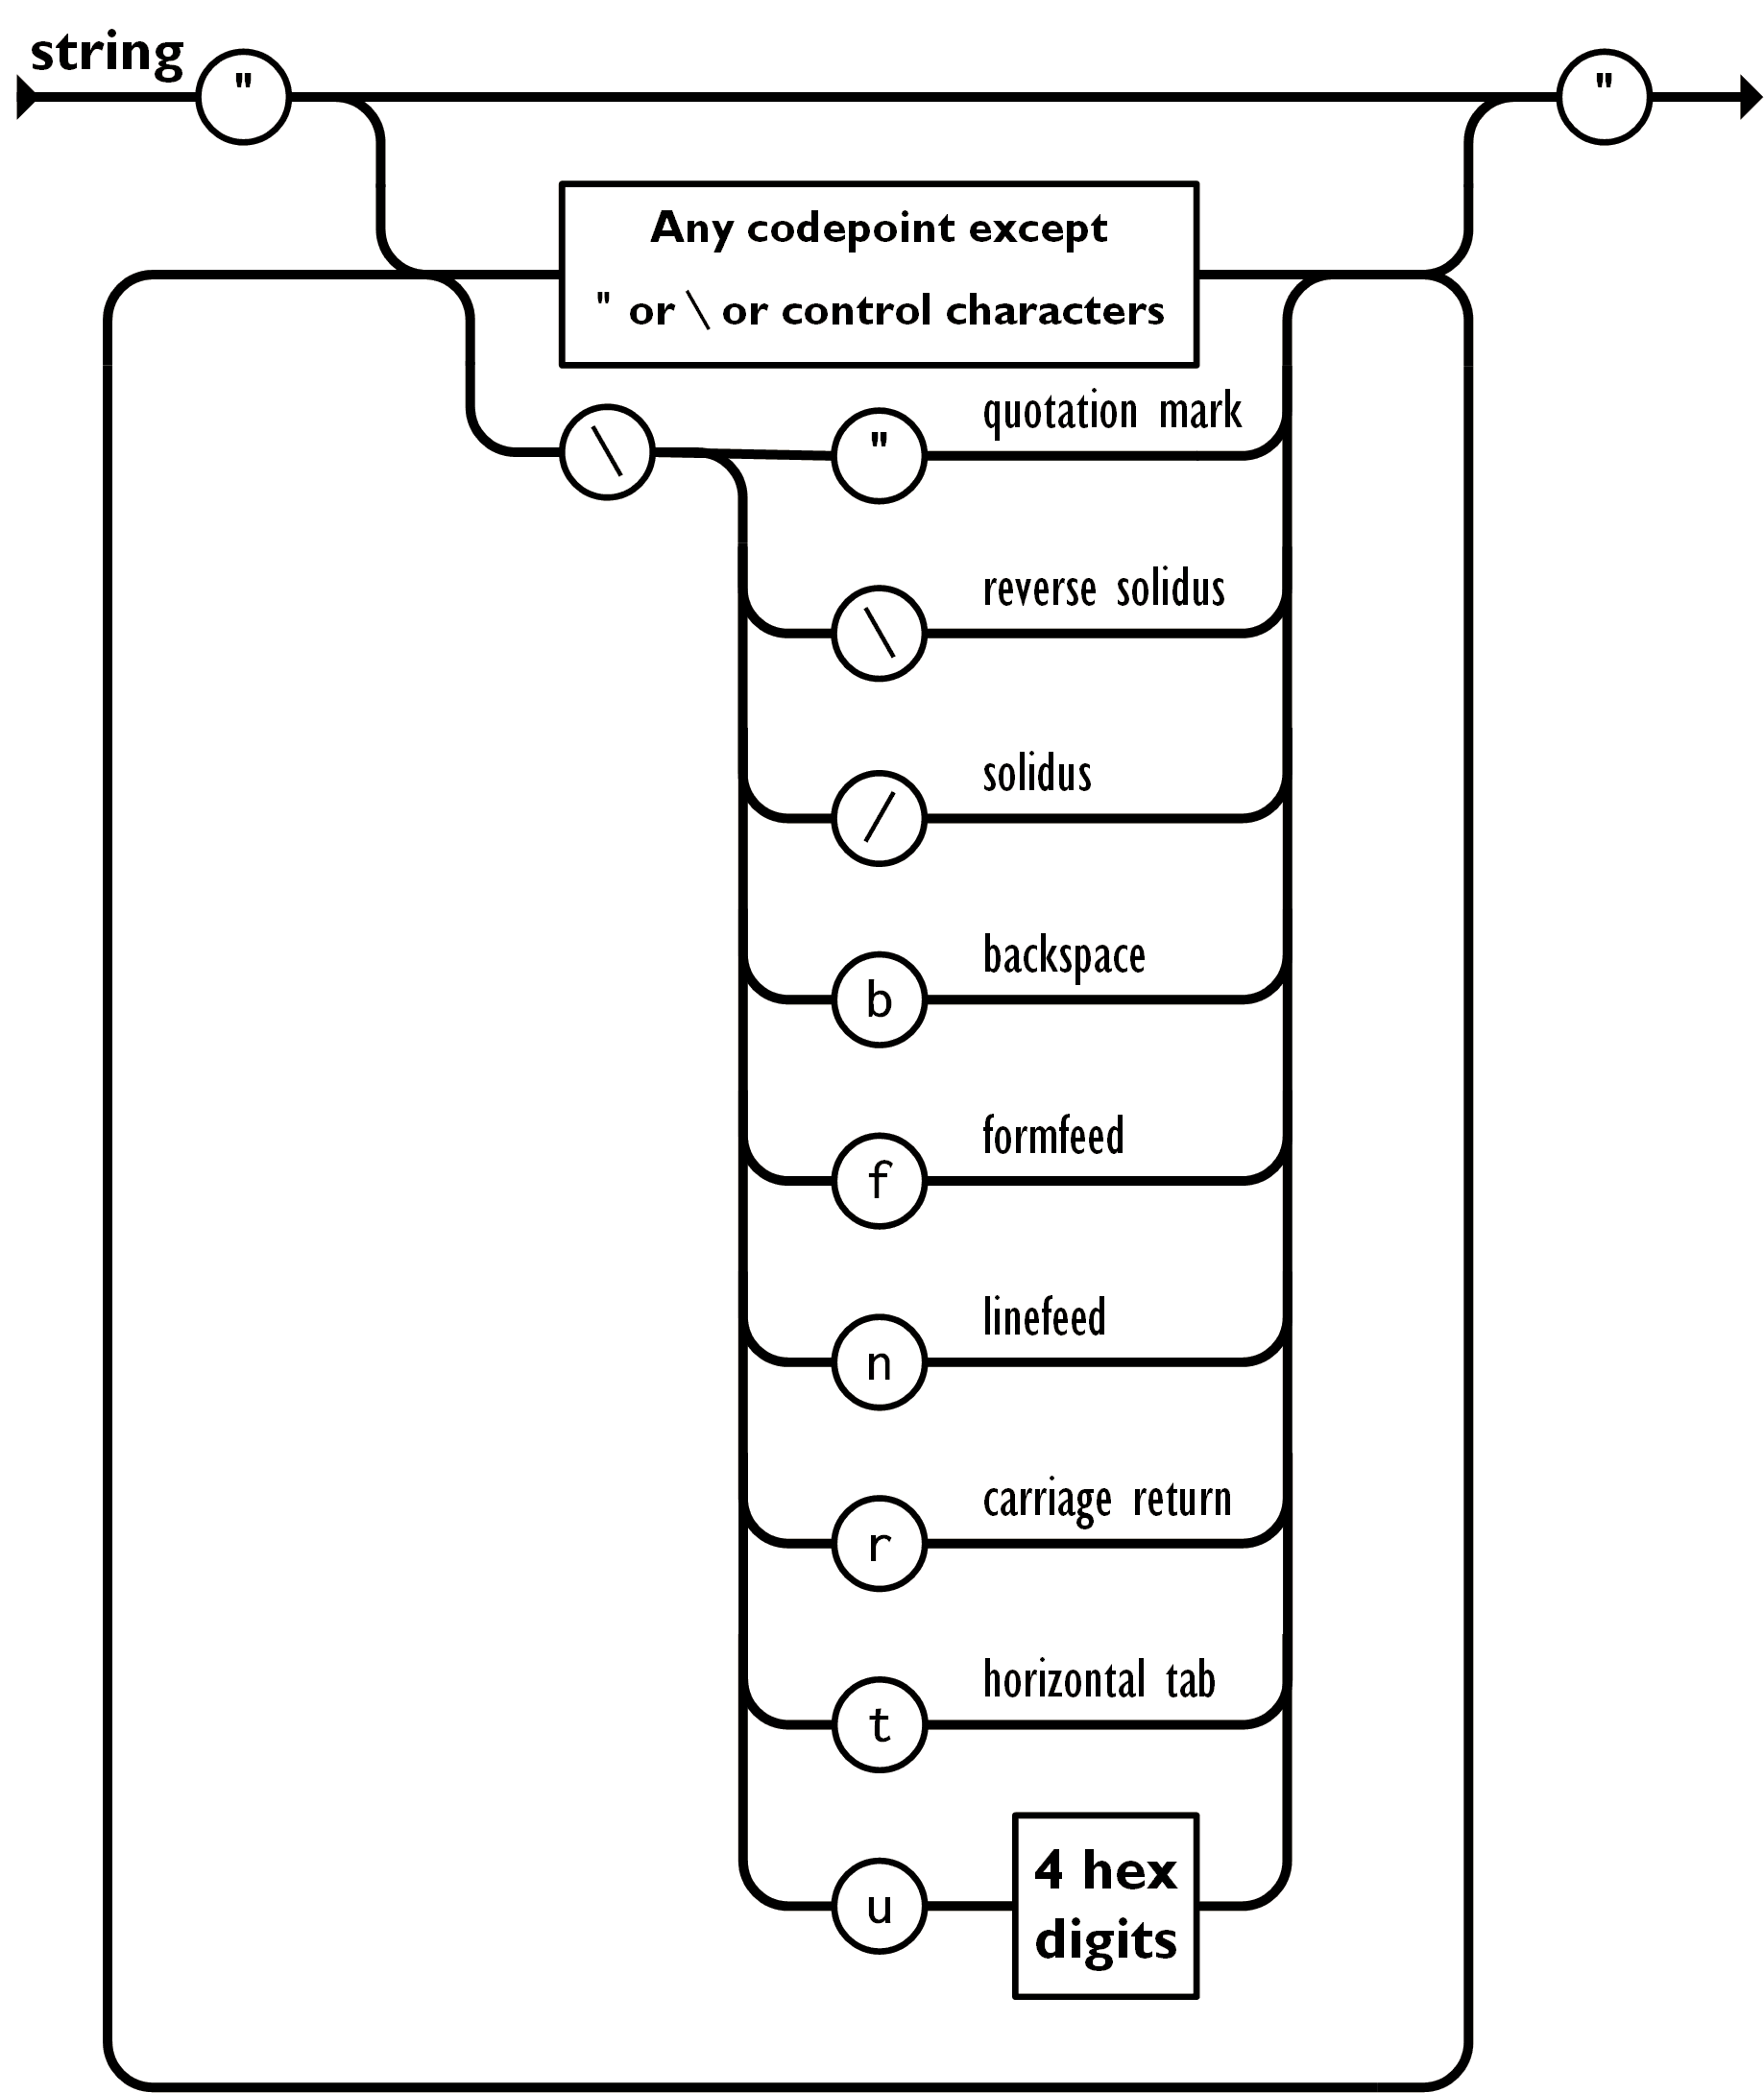
\includegraphics[scale=0.75]{jsonString}
    \caption[JSON String]{De structuur van een JSON string. \autocite{Crockford}}
    \label{fig:jsonString}
\end{figure}


\section{RESTful API}
\label{sec:RESTful API}

Representational State Transfer (REST) is zoals beschreven door \textcite{Fielding2000} een architecturale stijl voor het ontwerpen van gedistribueerde hypermediasystemen.

De combinatie van REST en API is een RESTful API, wanneer een RESTful API gecalled wordt dan zal de server een representatie van de huidige staat van de gevraagde resource weergeven.

\subsection{Design principes}
\label{subsec:Design principes}

Om een API als RESTful te kunnen beschrijven moet deze voldoen aan zes design principes die hieronder zullen worden verduidelijkt aan de hand van \textcite{Long} en \textcite{Naeem2021}

\textbf{Client-Server}

Dit principe zegt dat zowel de client als de server apart moeten kunnen worden ontwikkeld en moeten los staan van elkaar. Op deze manier wordt de handelbaarheid en schaalbaarheid aanzienlijk verbeterd aangezien de gebruikersinterface los staat van de gegevensopslag.


\textbf{Stateless}

Met stateless wordt bedoeld dat elke request die er naar de API gedaan wordt onafhankelijk is, een request heeft dus geen resultaat nodig van een andere request om te kunnen verder gaan. Met andere woorden moet de server geen vorige requests en states opslaan wat de benaming 'Stateless' verklaard.


\textbf{Cacheable}

Een REST API moet de mogelijkheid hebben om data te cachen, dit is het opslaan van data in digitaal geheugen. Volgens het Cacheable principe moet data in een response duidelijk gecategoriseerd worden als cacheable of non-cacheable. Indien een response cacheable is dan mag de cliënt cache deze data opslaan om gelijkaardige requests in de toekomst te beantwoorden.

\textbf{Uniform interface}

Om aan het client-server principe te voldoen is een uniforme interface nodig die autonome ontwikkeling van de applicatie mogelijk maakt zonder de acties, modellen en services te koppelen aan de API-laag. Door dit principe wordt de hele architectuur gestroomlijnd en wordt de visibiliteit van de communicatie verbeterd. Er zijn echter wel verschillende architecturale controles nodig die de performantie binnen de architectuur sturen om een uniforme interface te bereiken.

REST bevat vier interfacecontroles, namelijk: 

\begin{enumerate}
\item Identificatie van bronnen: Een Uniform Resource Locator (URL) identificeert de online locatie van een resource.
\item Beheer van bronnen door middel van representatie: Bronnen worden weergegeven aan de hand van media types ~\autocite{N.Freed1996} zoals JSON en XML.
\item Zelfbeschrijvende communicatie: Een bericht bevat alle informatie die de ontvanger nodig heeft om de informatie te begrijpen. Er mag geen extra informatie in een aparte documentatie of apart bericht zitten. Deze zelfbeschrijvende communicatie gebeurt door het gebruik van de accept en content-type HTTP headers die de inhoud die verzonden of aangevraagd wordt beschrijft.
\item Hypermedia: Hypermedia is data die verzonden wordt van de server naar de cliënt met informatie over wat de cliënt vervolgens kan doen. Hyper Text Markup Language (HTML) ~\autocite{W3schools} is hier een voorbeeld van.
\end{enumerate}

\textbf{Layered system}

De architectuur van een RESTful API bestaat uit verschillende lagen die door samen te werken een hiërarchie vormen die helpt bij het vormen van een flexibele, meer schaalbare applicatie. Dankzij het deze gelaagde structuur is de gevormde applicatie beter beveiligd, dit komt doordat componenten niet kunnen interageren buiten de eigen laag en de volgende laag. Daarnaast biedt het gedeelde caches aan die de schaalbaarheid verbeteren.

Deze gelaagde architectuur zorgt tot slot voor meer stabiliteit doordat het de componenten beperkt zodanig dat een component niet verder kan 'zien' als de laag waarmee het interageert.

\textbf{Code on demand}

Het 'Code on demand' principe zorgt ervoor dat codering kan worden gecommuniceerd via de API voor gebruik binnen de applicatie. De definitie van een RESTful API maakt het mogelijk dat functionaliteit aan de cliënt-kant kan worden uitgebreid door codering zoals applets of scripts te downloaden en te implementeren. Dit stroomlijnt cliënts door het aantal functies te verminderen die vooraf moeten worden geïmplementeerd.

Naast statische resources zoals XML en JSON kan dus ook uitvoerbare code aangeleverd worden door de server.

\textbf{Resources}

Bij REST kan elk stuk informatie een resource zijn, dit kan van alles zijn zoals documenten, services, collecties van andere resources, afbeeldingen, en dergelijke. In sommige gevallen wordt “Everything as a resource”  een zevende principe van REST genoemd. 

\subsection{Hoe werkt een RESTful API?}
\label{subsec:Hoe werkt een RESTful API?}

Zoals eerder vermeld in subsectie \ref{subsec:Design principes} heeft elke resource een unieke URL, zo een URL wordt een request genoemd waarbij de gereturnde data gekend staat als een response. In een RESTful API worden deze requests of transacties in vier componenten verdeeld zoals uitgelegd in REST API (cursus van Karine Samyn, 29 maart 2020, opleidingsonderdeel WebApplicaties IV).

\begin{itemize}
    \item \textbf{GET}: Deze request haalt een representatie van een resource op.
    \item \textbf{PUT}: Met PUT wordt een bestaande resource geupdatet.
    \item \textbf{POST}: Aan de hand van POST kunnen nieuwe resources en sub-resources aangemaakt worden.
    \item \textbf{DELETE}: De DELETE request gaat een reeds bestaande resource verwijderen.
\end{itemize}

\section{Protocol Buffers}
\label{sec:Protocol Buffers}

 In dit hoofdstuk zullen Protocol Buffers verduidelijkt worden, dit is het dataformaat dat gebruikt zal worden bij de implementatie van gRPC. In dit onderzoek zijn Protocol Buffers de tegenhanger van JSON.

\subsection{Wat zijn protocol buffers?}
\label{subsec:Wat zijn protocol buffers?}

Protocol buffers (protobuf) zijn net zoals JSON een manier om data te verzenden of op te slaan in bestanden en is ontwikkeld door Google zoals beschreven door \textcite{Kurian2020}. Een voorbeeld van een protobuf is te zien in figuur \ref{fig:protobufEx}.

\begin{figure}[H]
    \centering
    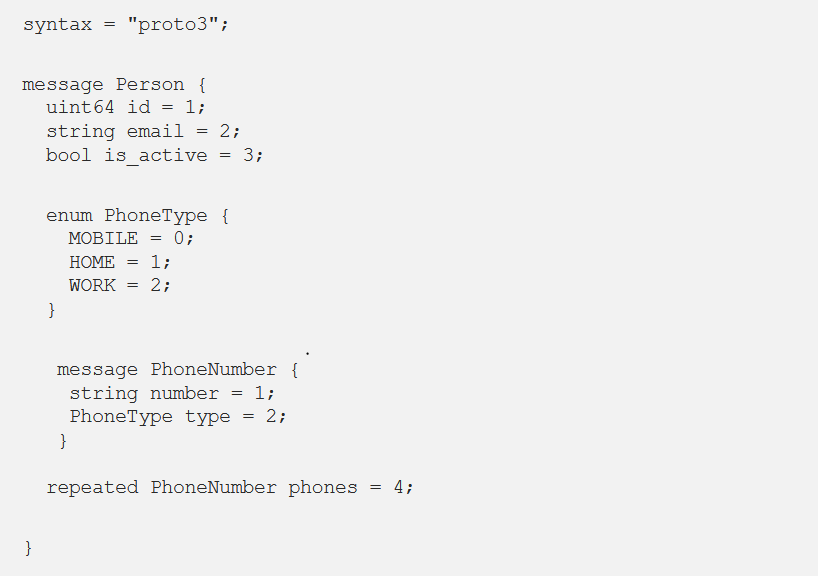
\includegraphics[scale=0.75]{protobufEx}
    \caption[Protocol Buffer .proto bestand]{Een voorbeeld van een .proto bestand.  \autocite{Kurian2020}}
    \label{fig:protobufEx}
\end{figure}

Formaten zoals JSON en XML zijn zeer flexibel maar zijn niet geoptimaliseerd voor het uitwisselen van data tussen meerdere microservices \autocite{Fowler2014} ongeacht het gebruikte platform. Protobuf is ontwikkeld met het oog op simpliciteit en performantie, om specifiek te zijn was het ontwikkeld om kleiner en sneller te zijn dan XML.

Protobuf onderscheidt zich van andere dataformaten door vele verantwoordelijkheden te verwijderen die normaal door het dataformaat aangepakt worden. Hierdoor gaat protobuf zich vooral focussen op het zo snel mogelijk serialiseren en deserialiseren van data. Daarnaast is een tweede optimalisatie de bandbreedte die gebruikt wordt door het zo klein mogelijk maken van de data die verzonden wordt.

Natuurlijk kunnen protobufs niet alleen voordelen hebben, een objectief nadeel dat protobuf heeft is dat het minder leesbaar is in vergelijking met JSON en XML.

Er bestaan meerdere versies van Protocol buffers, momenteel is de standaard protocol buffers versie 3 (proto3).


\subsection{Kerneigenschappen}
\label{subsec:Kerneigenschappen}

\textbf{Binair formaat}

Protobuf is een binair dataformaat, dit betekent dat de verzonden data omgezet wordt naar ééntjes en nulletjes. Deze eigenschap zorgt voor een verbetering van de transmissiesnelheid doordat het dataformaat minder bandbreedte en ruimte inneemt. Tot slot zorgt de omzetting van string naar binair formaat ook voor compressie, hierdoor zal het CPU gebruik ook lager zijn.

\textbf{Splitsing van context en data}

Zoals in \ref{fig:JSONsEx} te zien is maakt een formaat zoals JSON gebruik van key-value paren waar de data en de context in éénzelfde bestand zitten wat ook meer ruimte in beslag neemt. Bij protobuf is dit anders, hier worden data en context opgesplitst in een configuratiebestand ook wel gekend als een .proto bestand, waarin de message wordt gedefinieerd, zie figuur \ref{fig:protobufEx}, en geëncodeerde data die verzonden wordt aan de hand van het configuratiebestand.

\begin{figure}[H]
    \centering
    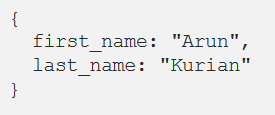
\includegraphics[scale=0.75]{JSONsEx}
    \caption[Simpel JSON key-value voorbeeld]{Een simpel voorbeeld van een key-value JSON bestand. \autocite{Kurian2020}}
    \label{fig:JSONsEx}
\end{figure}

\subsection{Message formaat}
\label{subsec:Message formaat}

Zoals hierboven vermeld is het configuratiebestand de plaats waarin de context gedefinieerd wordt, met andere woorden wordt hier de structuur van een bepaald object bepaald. Deze structuur wordt gedeclareerd door het “message” woord gevolgd door een zelfgekozen naam voor de message. Net zoals bij JSON worden de velden gedeclareerd binnen de accolades, deze velden kunnen elk in vier delen opgedeeld worden, namelijk veldregels, veldtypes, veldnamen en veldnummers \autocite{Google2020}.

\textbf{Veldregels}

In proto3 wordt enkel nog de “repeated” regel gebruikt, deze regel zegt dat de message dit veld meerdere keren mag bevatten met verschillende waarden. Met andere woorden, duidt dit op een array van een bepaald veldtype.

In proto2 waren er ook de required en optional regels. Required zorgt ervoor dat een message een bepaald veld exact één keer bevat en de optional regel zorgt ervoor dat een message een veld nul of één keer kan bevatten.

\textbf{Veldtypes}

Het field type is het datatype van een field, dit zijn er vier:

\begin{itemize}
    \item \textbf{Scalaire types}: Dit zijn de traditionele types zoals strings, integers, booleans, ...
    \item \textbf{Enum}: Binnen een message is het mogelijk om een attribuut te hebben dat enkel één van een aantal vooraf bepaalde waarden mag hebben.
    \item \textbf{Message types}: Net zoals bij andere dataformaten is het mogelijk dat een message andere messages als attribuut bevat.
\end{itemize}

\textbf{Veldnamen}

Veldnamen moeten volledig in kleine letters zijn en indien ze uit meerdere woorden bestaan moeten deze opgesplitst worden door een underscore. In tegenstelling tot JSON wordt hier dus geen camelcasing gebruikt. Deze conventies zijn vastgelegd omdat dit ook de conventies zijn die gevolgd worden door de Protoc compiler die code gaat genereren op basis van het .proto bestand.

\textbf{Veldnummer}

Elk veld heeft een uniek nummer, deze nummers worden gebruikt om de velden te identificeren in het binaire formaat. Als gevolg mogen deze niet veranderd worden eens het message type reeds gebruikt is.

\section{gRPC}
\label{sec:gRPC}

\subsection{Wat is gRPC?}
\label{subsec:Wat is gRPC?}

gRPC is open source Remote Procedure Call (RPC) framework en is in 2015 ontstaan uit zijn voorganger Stubby, deze was een single general-purpose RPC infrastructuur~\autocite{gRPC}. Deze technologie laat het toe voor een programma om procedures te starten op andere computers in, eventueel, verschillende ip-ranges aan de hand van een smal comminucatiekanaal~\autocite{Nelson1981}.

\subsection{Design Principes en requirements}
\label{subsec: Design Principes en requirements}

\textbf{Geen objecten maar services en Messages in plaats van Referenties}

Hiermee is het de bedoeling om de mircoservices design philosofie van coarse-grained berichtenuitwisseling te promoten zonder de problemen van gedistribueerde objecten \autocite{FowlerDisObj} en de valkuilen van het negeren van het netwerk \autocite{GalOz2008} te hebben.

\textbf{Coverage en Simpliciteit}

gRPC moet beschikbaar zijn op elk populair ontwikkelplatform en moet gemakkelijk zijn om op te bouwen op een platform naar keuze. Alsook moet gRPC werken op toestellen die CPU en geheugen gelimiteerd zijn.

\textbf{Gratis en Open}

De fundamentale features van gRPC zijn gratis om te gebruiken en  alle artifacten worden gereleased als open-source efforts, hierbij moet licensing er voor zorgen dat het aannemen van het framework wordt vergemakkelijkt en niet vermoeilijkt.

\textbf{Interoperabiliteit en Bereik}

Het wire protocol moet zonder problemen kunnen reizen doorheen de internet infrastructuur.

\textbf{Algemeen Doel en Performant}

De stack moet bruikbaar zijn in een grote aanbod van use-cases zonder dat performantie verloren gaat ten opzichte van specifieke stack voor die use-case.

\textbf{Gelaagd}

Onderdelen van de stack moeten zich individueel evolueren, bij het updaten van het wire-formaat met het vernieuwde onderdeel mogen de bindingen tussen de applicatielagen niet verstoord worden.

\textbf{Payload Agnostisch}

gRPC en de implementatie ervan zorgen ervoor dat elke service  een andere message type en encoding systeem kan gebruiken zoals protocol buffers en JSON. Alsook zorgt gRPC er voor dat verschillende payload compressie mechanismes kunnen gebruikt worden aangezien deze kunnen verschillen per use-case.

\textbf{Streaming}

gRPC moet bruikbaar zijn met streaming, onder andere opslagsystemen maken hier gebruik van samen met flow control om grote data-sets uit te drukken. Er zijn ook andere services zoals voice-to-text die afhankelijk zijn van streaming voor berichtsequenties te representeren die een tijdelijke relatie hebben met elkaar. Streaming is enkel mogelijk dankzij het gebruik van het HTTP/2 protocol \autocite{Grigorik2013} 

\textbf{Blocking en Non-Blocking}

gRPC ondersteunt zowel asynchrone als synchrone processing van de data uitwisseling tussen client en server. Dit requirement is van groot belang op vlak van schaalbaarheid en het omgaan met streams.

\textbf{Annulering en Timeout}

Doordat sommige operaties lang en “duur” kunnen zijn op vlak van resources laat annulering het toe voor een server om de resources terug ter beschikking te zetten wanneer clients zich goed gedragen. Annulering kan ook cascaden wanneer een causale keten is gedetecteerd.

\textbf{Lameducking}

Een server moet zich kunnen afsluiten door reeds lopende requests af te werken maar geen nieuwe requests meer te accepteren.

\textbf{Flow Control}

Flow control zorgt voor betere buffer management dat kan ontstaan door een onevenwichtige balans van computing power en netwerk capaciteit tussen client en server. Als ook biedt flow control bescherming tegen DOS door een over actieve peer.

\textbf{Pluggable}

Een wire protocol zoals gRPC is enkel een onderdeel van een API infrastructuur. Implementaties van gRPC moeten extensiepunten voorzien voor het inpluggen van features zoals logging, health-checking, tracing,... en indien nuttig een basis implementatie van de feature.

\textbf{Extensies als APIs}

Extensies waarvoor een samenwerking tussen meerdere services nodig is moeten de voorkeur hebben van een API te gebruiken in plaats van protocol extensies. Voorbeelden van zulke extensies zijn health-checking en load-monitoring.

\textbf{Metadata uitwisseling}

Zaken zoals authenticatie zijn afhankelijk van het gebruik van metadata, dit is data die geen onderdeel is van de gegevensuitwisseling die gedefinieerd is in de interface of service.

\textbf{Gestandaardiseerde statuscodes}

Er zijn voor de client maar een gelimiteerd aantal manieren voor het omgaan met error die verkegen zijn van de API. Om de error handling beslissingen duidelijker te maken moet de statuscode namespace afgebakend worden, indien er meer specifieke statussen nodig zijn kan hiervoor metadata gebruikt worden.

\subsection{Werking van gRPC}
\label{subsec: Werking van gRPC}

Bij gRPC kan een client applicatie een bepaalde methode die op een remote server draait rechtstreeks aanspreken alsof het een lokaal object zou zijn, dit maakt het gemakkelijk voor het gebruiken van distribueerde applicaties en services.

gRPC definieert net zoals in vele RPC systemen, een service waarin de methodes die kunnen worden aangeroepen worden gespecificeerd samen met hun parameters en return types. Deze interface wordt op de server geïmplementeerd en draait een gRPC server om client calls af te handelen. De client heeft een stub die dezelfde methodes als de server bevat.

Op deze manier kunnen gRPC servers en clients draaien en tegen elkaar praten in verschillende omgevingen. Dit laat het bijvoorbeeld toe om een gRPC server in C\# te draaien met clients die draaien in Python.

Standaard worden door gRPC Protocol Buffers gebruikt, hierbij worden de services gedefinieerd in ordinaire proto bestanden met RPC methode parameters en return types als protocol buffer messages. Aan de hand van het protoc commando samen met een gRPC plugin wordt automatisch client en server code gegenereerd op basis van het proto bestand samen met de standaard protobuf code voor het populeren, serialiseren en ophalen van de gespecificeerde message types.


\section{Interne architectuur Fashion Society}
\label{sec:Interne architectuur Fashion Society}

De Fashion Society werkt met een architectuur gebouwd rond microservices, om de gehele flow binnen de architectuur te garanderen is deze gebaseerd op basis van enkele design patronen. Om de architectuur te verstaan zullen de design patronen die van toepassing zijn in deze bachelorproef kort uitgelegd worden aan de hand van hun huidige toepassing.

\subsection{Microservice architectuur patroon}
\label{subsec:Microservice architectuur patroon}

Dit patroon zegt dat de architectuur bestaat uit meerdere los van elkaar staande, samenwerkende services waarin elke service:
 \begin{itemize}
     \item Onderhoudbaar en testbaar is. Hierdoor kunnen services snel aangepast en gedeployed worden.
     \item Los verbonden is van andere services, dit zorgt ervoor dat elke service kan draaien zonder beïnvloed te worden door veranderingen in andere services.
     \item Zelfstandig deployable is.
     \item Ontwikkelbaar door een klein team.
 \end{itemize}
\autocite{Richardsonc}

Binnen de Fashion Society wordt aan elk van deze requirements voldaan en communiceren de services aan de hand van HTTP/REST protocollen.

\subsection{API-gateway patroon}
\label{subsec:API-gateway patroon}

 In dit patroon wordt gedefinieerd dat de architectuur een API gateway heeft. Deze is het enige entry point voor alle clients \autocite{Richardsonb}.
 
 Dit patroon staat bij de Fashion Society in nauwe samenwerking met het Service registry patroon en het Self Registration patroon en wordt de Orchestrator genoemd.De Orchestrator heerst en verdeelt over de micro services, elke request, inclusief de interne requests tussen APIs moeten via de Orchestrator verlopen.
 
 \subsection{Service Registry patroon}
 \label{subsec:Service Registry patroon}
 
 Het Service Registry patroon zegt dat de architectuur een service registry bevat, dit is een database van services en hun gegevens. \autocite{Richardsona} Bij de Fashion Society is dit de een SQL database die aan de Discovery API hangt en de servicenaam, server en poort bevat. Deze database wordt aangeroepen door de endpoints in de Discovery API. Deze aanroepingen gebeuren aan de hand van requests die de gegevens van een bepaalde service kunnen opvragen zoals de url van de locatie van een service of het volledige service object.
 
 \subsection{Self Registration patroon}
 \label{subsec:Self Registration patroon}
 
 Elke instantie van een service is zelf verantwoordelijk om bij het opstarten zichzelf te registreren bij de Service Registry. \autocite{Richardson}
 
 In de Startup klasse van elke service zit er een stuk code waarin de service zich gaan aanmelden bij de Discovery API aan de hand van een POST request zijnde RegisterService, dit gebeurt enkel wanneer er in een online omgeving wordt gewerkt zoals de test, UAT en live omgevingen, dit is om te voorkomen dat een bepaalde service al beschikbaar is in de Discovery API maar in realiteit nog niet draait.
 
 \subsection{SOLID Principes}
 \label{subsec:SOLID Principe}
 
 De SOLID principes zijn een onderdeel van Object-Oriented Programming en zijn vijf richtlijnen voor het ontwikkelen van software zodanig dat deze eenvoudiger zijn om te onderhouden en eventueel te schalen. Hieronder een verduidelijking van elke letter in het woord SOLID. \autocite{Thelma}
 
 \textbf{Single Responsibility}
 
 Het eerse principe is single responsibility, dit principe zegt dat een klasse of in de context van deze bachelorproef, een micro-service maar één verantwoordelijkheid mag hebben. Naar mate een klasse of service meer verantwoordelijkheden heeft, wordt her risico bij het aanpassen van een verantwoordelijkheid groter dat een bug opduikt bij een andere verantwoordelijkheid. 
 
 Dit principe gaat gepaard met punt twee van sectie \ref{subsec:Microservice architectuur patroon} dat zegt dat elke service los verbonden moet zijn van andere services.
 
 Een customer service mag dus geen data behandelen dat te maken heeft met vouchers, dat is de taak van de voucher service.
 
 \textbf{Open-Closed}
 
 Een klasse of service moet open zijn voor uitbreiding maar gesloten voor aanpassing. Het gedrag van een bepaalde endpoint in een service mag niet zomaar aangepast worden, dit heeft namelijk invloed op alle services of applicaties die deze endpoint gebruiken. Indien een endpoint van een service extra functionaliteit moet hebben is het beter om een nieuwe endpoint aan te maken die voor deze extra functionaliteit zorgt.
 
 Het doel van dit principe is om extra functionaliteit te voorzien zonder problemen te veroorzaken bij services of applicaties waar de huidige functionaliteit gebruikt wordt.
 
 \textbf{Liskov Substitution}
 
 Als een klasse S van een bepaald subtype T is dan kunnen klasses van type T vervangen worden door klasses van type S zonder dat het invloed heeft op de propeties van het programma.
 
 Concreet wil dit zeggen dat als een klasse overerft van een andere klasse, deze minstens hetzelfde moet kunnen doen als de ouder. Dit principe heeft als doel om consistentie te verzekeren doorheen een programma, zodanig dat een kind klasse en ouder klasse foutloos op dezelfde manier kunnen gebruikt worden.
 
 \textbf{Interface Segregation}
 
 Het is beter om meer specifieke interfaces te hebben dan één algemene interface. Een client zou geen methodes moeten implementeren die deze niet gebruikt. Het implementeren van methodes die niet gebruikt worden en dus nutteloos zijn heeft als grootste nadeel dat deze onverwachte bugs kunnen creëren.
 
 Met andere woorden moet een klasse enkel methodes implementeren die nodig zijn voor uitvoeren van zijn taken, andere methodes die niet van toepassen zijn moeten dus verwijderd worden of verplaatst naar een andere interface indien ze gebruikt worden door een andere klasse.
 
 Het doel hiervan is om methodes op te splitsen in meerdere interfaces zodanig dat een klasse enkel de methodes moet implementeren die hij nodig heeft.
 
 \textbf{Dependency Inversion}
 
 Tot slot is er Dependency Inversion, dependency inversion zegt dat men niet afhankelijk moet zijn van implementaties maar van abstracties. Dit kan bereikt worden door het gebruik van Dependency Injection \autocite{Ilyana}.
 
 Het doel van Dependency Inversion is om de afhankelijkheid van een high-level klasse op een low-level klasse te beperken. Beide moeten afhankelijk zijn van abstracties.
 
 
 
 \subsection{Algemene werking voorbeeld}
 \label{subsec:Algemene werking voorbeeld}
 
 Een personeelslid van team Customer Service wil graag een klant opzoeken om deze verder te helpen. Hij geeft de gegevens in in een tool die klanten ophaalt, dit is nu de Client. 
 
 De Client komt binnen bij de Orchestrator met de request om een bepaalde klant op te halen, in deze request zit ook de naam van de benodigde API, zijnde de CustomerAPI. Vervolgens stuurt de Orchestrator een request naar de DiscoveryAPI voor de gegevens van de gevraagde API, de DiscoveryAPI zal deze request beantwoorden met de server en poort waarop de CustomerAPI te vinden is. 
 
 Vervolgens kopieert de Orchestrator de originele request van de Client naar een nieuwe call die wordt verzonden naar de CustomerAPI op basis van de verkregen server en poortnummer. Deze call zal dan beantwoord worden met de juiste klantgegevens en gaat via de Orchestrator terug tot bij de Client. 
 
 Dit gehele proces kan gevolgd worden in figuur \ref{fig:CSFlow}
 
 \begin{figure}[H]
     \centering
     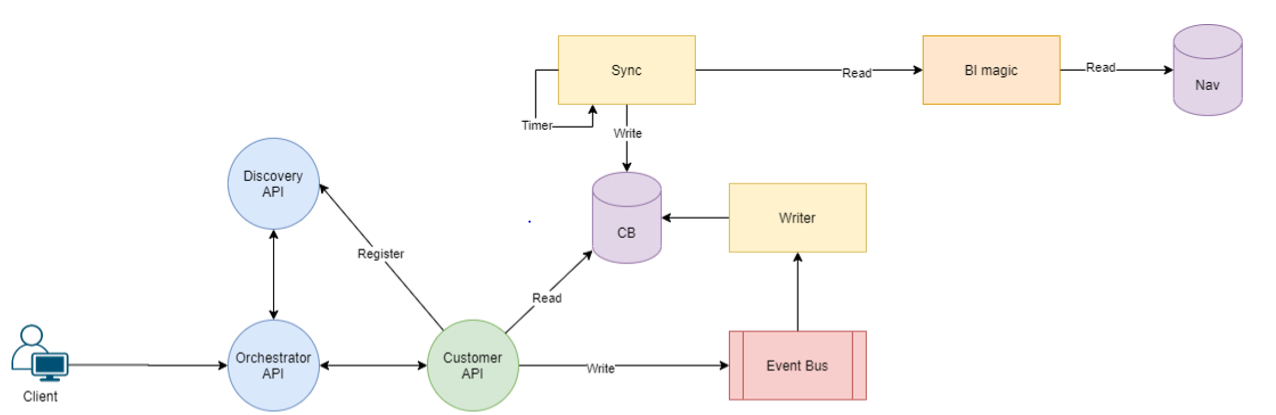
\includegraphics[scale=0.5]{CSFlow}
     \caption[Customer Service Dataflow]{De interne werking voor het afhandelen van klantengegevens}
     \label{fig:CSFlow}
 \end{figure}
 
 
 
 







